

\subsection{Introdução}
		Com o avanço da tecnologia RFID e o crescente interesse popular e industrial por esta tecnologia, a área de TI tem sido desafiada a criar recursos que permitam a interface e integração com sistemas RFID. Cada tag em um sistema RFID possui uma identificação única (UID) e os que possuem memória são capazes de gravar informações sob demanda.
	
		Devido a popularidade dos RFID, foram propostas muitas aplicações. Por meio do sinal sem fio de curta distância, usuários de uma tag RFID podem ser monitorados dentro de uma área específica. Assim, sistemas RFID são normalmente utilizados para identificação de um hardware ou objeto em muitas aplicações. Muitas dessas aplicações são baseadas em ambientes internos ou pequenas áreas de serviço independentes do sistema utilizado.
	
		Aplicações RFID vão além de códigos de barra ou banco de dados portáteis. RFID pode ser utilizado para a Segurança da Cadeia de Suprimentos (SCS) e gestão da vida útil de equipamentos ou alimentos. Como exemplo podemos citar o envio de toneladas de rações do Exército dos Estados Unidos para as tropas no Iraque e em outras localidades do mundo. Estas transferências são feitas por navios, que carregam milhares de contêiners padronizados. Como o Exército dos EUA faz para garantir que essa transferência foi esquecida, adulterada ou exposta a condições ambientais inapropriadas? Eles utilizam a tecnologia RFID integrada com sofisticados sensores para uma uma série de eventos ambientais, tais como: temperatura, radiação, luz, agentes químicos, agentes biológicos, choque, sensores de portas, entre outros. Se alguém esta fazendo algo com o carregamento de comida, ou se ela apenas fica quente por muito tempo, o Exército dos Estados Unidos conseguem saber onde e quando esse evento ocorreu. Esta é apenas uma aplicação entre tantas outras de tecnologia RFID em uma organização, no nosso exemplo, o Exército dos EUA. Atualmente a maior barreira para a implantação e adoção de sistemas RFID é a integração com sistemas legados [3].
		
		
		\begin{figure}[h!]
			\centering
				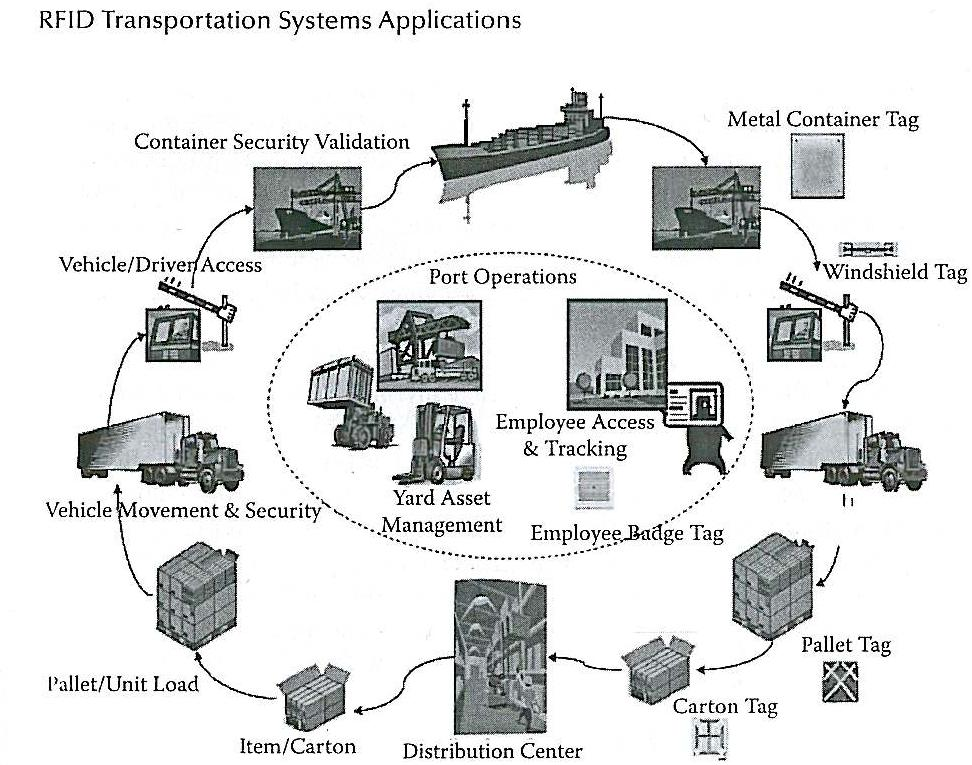
\includegraphics[width=0.7\linewidth]{Ex1SCS.jpg}
			\caption{Transporte de Alimentos monitorado por RFID}
			\label{fig:Ex1SCS}
		\end{figure}
		
	
	
		Alguns sistemas RFID foram propostos para serem utilizados em hospitais ou para cuidados da saúde[1]. Cada paciente recebe uma etiqueta (tag) RFID projetada. O paciente deverá usa-la constantemente, não importando o lugar nem o horário. Assim a localização e condições de saúde atuais do paciente poderão ser monitorados pelo hospital.
	
		Como RFID geralmente é utilizado para identificação, ele também pode ser utilizado em aplicações que usam criptografia de softwares como as identificações para proteger a propriedade intelectual de aplicativos ou arquivos. Algumas pesquisas mostram que o RFID pode ser incorporado em pequenos dispositivos. Os usuários do dispositivo podem conectar uma interface SD de leitor de cartão RFID. Dessa maneira os usuários poderão digitalizar e introduzir o RFID em todos os lugares. Uma vez que sistemas RFID fazem tratamento distintivo de um alvo individual, a caracterísitica única ou identificação RFID pode ser uma solução para a proteção da propriedade intelectual.
	
		Como se pode perceber esse conjunto de tecnologias baseadas em radiofrequência abriram uma ampla gama de possibilidades e oportunidades de forma direta e integrada para diferentes campos e áreas técnicas. Requisitos para efetiva implementação do sistema RFID exigem produtos específicos RFID, serviços e soluções de acordo com a escala e exigência do negócio.
		
		Dada a grande variedade de sistemas RFID, torna-se necessário o desenvolvimento de ferramentas de integração flexíveis, independentes de sistema operacional.
		
		
	
		
\subsection{Integração}
		O próprio leitor de RFID não pode lidar com a informação coletada de forma independente, tornando-se essencial a integração com outros sistemas ou ser agregado em aplicações existentes. Primeiramente, o designer do aplicativo tem que saber se a integração do aplicativo é baseada em software, hardware ou ambos. Se for um novo sistema, RFID poderá ser diretamente incorporado nele. No entanto, se a integração for com um sistema que ja existia, uma interface deverá ser decidida e definida.
		
		
\subsection{Vantagens da integração}
		Tecnologia RFID possui muitas características que a torna interessante e viável para integração com uma grande variedade de aplicações na industria, consumidores e comércio. Para integrar sistemas RFID eficientemente, é necessário a cooperação multidisciplinar de profissionais da área de TI, gestão de processos, projetistas de sistema, entre outros. Os RFIDs são mais ricos de informação do que os tradicionais códigos de barras. As etiquetas (ou tags) RFID geram valor ao produto pelas seguintes características:
		
		
		\begin{itemize}
			\item RFID não necessita de leitura visual, podendo realizar a leitura do objeto de dentro da caixa;
			\item Recurso de leitura/escrita criptografadas com usuários requeridos no armazenamento de dados;
			\item Monitoramento em tempo real por meio da internet/intranet para controle de estoques, redução de desperdícios e integração mais apertada da cadeia de suprimentos;
			\item Identificação automática por meio de redes sem fio;
			\item Podem sobreviver vários anos em ambientes hostis;
			\item Vários tipos de leitores de tags RFID estão disponíveis, como antenas inteligentes e impressoras portáteis.
		\end{itemize}
		
	
\subsubsection{Processo de Integração RFID}
Integração de sistemas RFID eficiênte exige conhecimentos abrangentes e a compreensão de diferentes sistemas. Para integrar funções RFID dentro de um sistema com outras tecnologias, como scan, controle e tecnologia da informação exige conhecimento e experiência com integração e hardware.


\begin{figure}[h!]
	\centering
		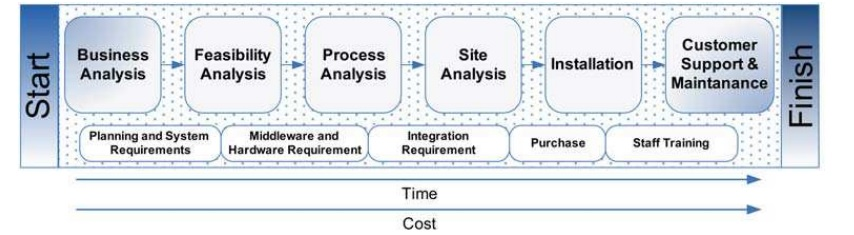
\includegraphics[width=0.7\linewidth]{etapas_integracao.jpg}
	\caption{Etapas para o projeto de Integração de Sistemas RFID.}
	\label{fig:etapas_integracao}
\end{figure}


		Cada projeto de negócio tem seus próprios requisitos e obstáculos técnicos que exige personalização de sistemas RFID. Deve-se, primeiramente fazer uma análise de viabilidade do meio. Para resolver eventuais problemas é aconselhado fazer a instalação de RFID em etapas. No processo de implementação cada etapa poderá ser revisada. Em alguns ambientes, leitores RFID móveis podem ser utilizados para aumentar ou substituir modelos estacionários.
		Para aumentar a confiabilidade deve-se fazer um planejamento e implementação de reconfigurações, gravação otimizada, segurança e autentificação.
		

\subsubsection{Componentes para Integração com Sistemas RFID}
Além dos componentes básicos de um sistema RFID, como tag, leitor e middleware, outros componentes também devem se levados em consideração para ser feita a integração. A figura abaixo apresenta o esquemático dos componentes necessários para a integração:


\begin{figure}[h!]
	\centering
		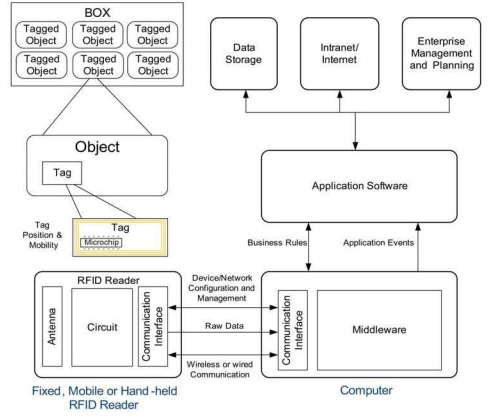
\includegraphics[width=0.5\linewidth]{componente integracao.jpg}
	\caption{Componentes para Integração de RFID.}
	\label{fig:componente integracao}
\end{figure}


\subsubsection{Posição e Mobilidade da Tag}
Este fator é necessário ser levado em consideração para obter uma melhor performance do sistema. Quando a tag ou o leitor estão se movendo, trata-se de mobilidade. Para poder garantir a identificação da tag, a velocidade do movimento deve ser levada em consideração.
		
		A decisão da posição da tag é crítico para tags passivas. Essa escolha deve levar em consideração a Potência Efetiva Radiada, que pode ter efeitos como ressônancia do sinal e morte do sinal.
		
		
\subsubsection{Módulos de Comunicação}
Diferentes formas de conexão podem ser utilizados, com ou sem fio. Padrões e normas variados podem ser utilizados, dependendo  do tipo de comunicação: com/sem fio, tipo de conector, custo, alcance, requisitos de segurança de aplicativos, entre outros.


\subsubsection{Aplicativos de Software para Integração de Sistemas}
Aplicativos de software executam em computadores comuns ou servidores e que comunicam com o middleware, controladores e dados de equipamentos de automação podendo realizar o controle das operações do Workflow.

		Os sistemas RFID exigem software que gerencia dispositivos, dados, rede e processos para permitir um fluxo contínuo de informação, alertas e respostas em tempo real.

		
\subsubsection{Servidor para Gravação de Dados}
	Usando uma apropriada infra-estrutura de rede, os dados obtidos de middleware podem ser gravadas e utilizadas para o desenvolvimento, implantação e manutenção de soluções produtivas. O servidor central executa aplicação de banco de dados com funções que incluem correspondência, rastreamento e armazenamento.


\subsubsection{Integração de RFID com simples Circuito}
Muitos sistemas de controle mecânico simples tem seu hardware baseado em projeto de circuitos. De acordo com a exigência ou ação da máquina, algumas ações mecânicas são acionadas quando recebem um sinal de On/Off. O leitor do sistema RFID atua como um fio elétrico para a transmissão de sinal para o circuito simples.


		\begin{figure}[h!]
			\centering
				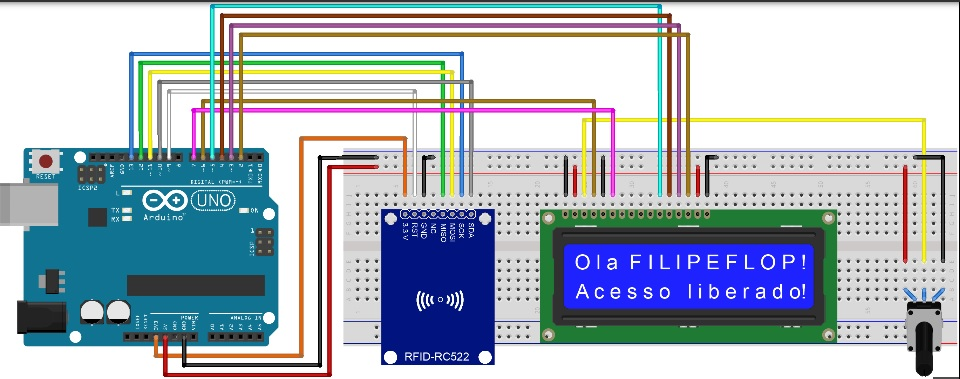
\includegraphics[width=0.7\linewidth]{mosfet_rfid.jpg}
			\caption{Exemplo de Circuito integrado a RFID.}
			\label{fig:mosfet_rfid}
		\end{figure}
		

		Neste tipo de integração, o sistema RFID funciona como um emissor de sinais. Quando o leitor de RFID induz as tags RFID, o leitor verifica se o tag RFID induzida é a tag pré-definida ( por exemplo, como válida) ou não. Se a tag induzida for uma pré-definida, o leitor envia o sinal de controle para acionar o hardware ou ação mecânica tal como abrir a porta de bloqueio. Dessa forma o sistema integrado vai agir com base na decisão do sistema RFID.
		
		
\subsubsection{Porta Serial RS-232}
O RS-232 consiste de dois dispositivos: DTE e DCE. Ao enviar sinal de controle, os dispositivos podem comunicar entre si via cabo RS-232. De acordo com o padrão de comunicação RS-232, o leitor do RFID pode enviar comandos pré-definidos através de RS-232 para acionar uma máquina ou sistema; ou então enviar um sinal emulado como comando para acionar os sistemas. Neste tipo de integração o RFID, pode exercer as seguintes funções: servir como um fio elétrico que aciona sistemas ou ser atuar como uma unidade computacional simples (IC chip) para o controle da porta serial e o comando de ordenação.


\subsubsection{USB e Acesso à internet}
Dependendo do hardware do computador, o leitor de RFID pode se conectar ao computador via porta USB ou conexão RJ45 Internet. Quando se conecta via USB, a informação da tag RFID pode ser transmitida para o PC diretamente. As aplicações que recebem informações do leitor RFID podem melhorar as funções ou capacidades dos serviços. O sinal de controle, a função de execução, ou ainda a gestão da informação podem ser feitos pelos aplicativos.

		Se a comunicação é através da internet, o leitor de RFID tem, pelo menos, o componente de rede e uma unidade de processamento central de informações suficientes para a computação. O sistema RFID funcionará como um dispositivo de rede pertencente a rede da plataforma, podendo agir de forma independente. O acesso pelo cabo de Internet é apenas para transmissão de dados e informações.
		
		Não importa se a comunicação é com base na porta USB ou pela conexão de rede, o sistema RFID tem apenas o papel de coleta informações.




\subsection{Considerações Finais}
Nesta seção foram vistos diversos exemplos de situações em que são ou podem ser empregados a integração de sistemas RFID. Também foram vistos os componentes necessários para permitir essa comunicação.
Por fim o capítulo apresentou diferentes conexões com fio entre o sistema RFID e um dispositivo, geralmente um computador.

		
	